\documentclass[12pt, a4paper]{article}

\usepackage[utf8]{inputenc}
\usepackage{amsmath, amssymb}
\usepackage{graphicx}
\usepackage{geometry}
\usepackage{tikz}
\usetikzlibrary{shapes, arrows, positioning}

\geometry{top=1in, bottom=1in, left=1in, right=1in}

\title{\textbf{Adaptive Fault-Tolerant Control of an Octorotor \\ Paper Understanding Report}}
\author{Agolika \\ IISc Internship}
\date{\today}

\begin{document}

\maketitle

\section{Introduction}
The paper addresses the challenge of keeping an 8-rotor drone (coaxial octorotor) flying safely even when multiple motors fail at the same time. Instead of relying on a separate system to detect and isolate faults (which is slow and complex), the paper uses a robust approach: an \textbf{Adaptive Sliding Mode Controller (ASMC)} to handle uncertainty, paired with a \textbf{Control Allocation} strategy to dynamically distribute the required effort across the remaining healthy motors.

\section{System Architecture: Inputs, Outputs, and States}
To understand the system, we must define what the controller "sees" and "commands".

\subsection{State Vector}
The state of the drone describes its position and orientation in 3D space. It is represented by an 8-dimensional vector:
\[
\mathbf{X} = [z, \dot{z}, \phi, \dot{\phi}, \theta, \dot{\theta}, \psi, \dot{\psi}]^T
\]
where $z$ is altitude, and $\phi, \theta, \psi$ are the roll, pitch, and yaw angles (with their respective velocities). 

\subsection{Inputs and Outputs}
The control system operates in two stages, creating distinct sets of inputs and outputs:
\begin{itemize}
    \item \textbf{Virtual Control Inputs ($\nu$):} The high-level ASMC calculates the total forces needed to stabilize the drone. This is a 4-dimensional vector: $\nu = [U_z, U_\phi, U_\theta, U_\psi]^T$ (Total Thrust, Roll Torque, Pitch Torque, Yaw Torque).
    \item \textbf{Actual Motor Commands ($u$):} The low-level Control Allocation module takes the 4 virtual inputs and converts them into 8 individual motor thrust commands: $u = [u_1, u_2, \dots, u_8]^T$.
    \item \textbf{System Output ($y$):} The physical response of the drone (Altitude and Attitude), which is fed back into the controller to close the loop.
\end{itemize}

\section{Closed-Loop System Diagram}

Below is the closed-loop control architecture representing the paper's methodology:

\begin{figure}[H]
    \centering
    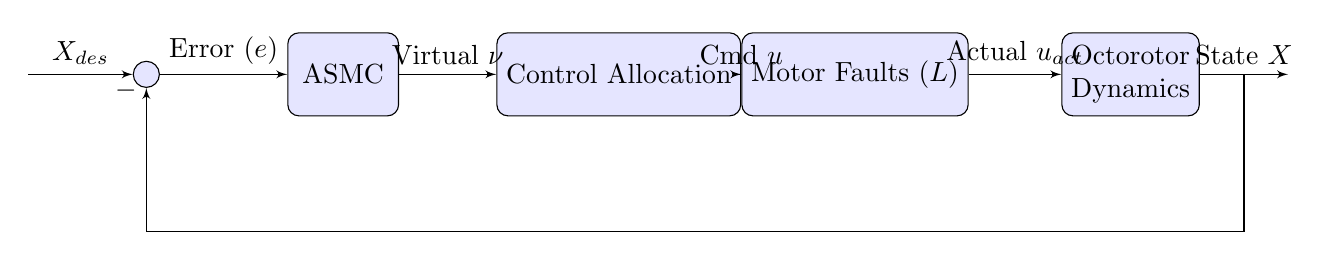
\begin{tikzpicture}[auto, node distance=2cm, >=latex']
        % Define block styles
        \tikzstyle{block} = [draw, fill=blue!10, rectangle, minimum height=3em, minimum width=4em, text centered, rounded corners]
        \tikzstyle{sum} = [draw, fill=blue!10, circle, node distance=1.5cm]
        \tikzstyle{input} = [coordinate]
        \tikzstyle{output} = [coordinate]
        
        % Nodes
        \node [input, name=ref] {};
        \node [sum, right of=ref] (sum) {};
        \node [block, right of=sum, node distance=2.5cm] (asmc) {ASMC};
        \node [block, right of=asmc, node distance=3.5cm] (ca) {Control Allocation};
        \node [block, right of=ca, node distance=3cm] (faults) {Motor Faults ($L$)};
        \node [block, right of=faults, node distance=3.5cm, align=center] (drone) {Octorotor \\ Dynamics};
        \node [output, right of=drone, node distance=2cm] (out) {};
        \node [coordinate, below of=ca, node distance=2cm] (feedback) {};

        % Edges
        \draw [->] (ref) -- node {$X_{des}$} (sum);
        \draw [->] (sum) -- node {Error ($e$)} (asmc);
        \draw [->] (asmc) -- node {Virtual $\nu$} (ca);
        \draw [->] (ca) -- node {Cmd $u$} (faults);
        \draw [->] (faults) -- node {Actual $u_{act}$} (drone);
        \draw [->] (drone) -- node [name=y] {State $X$} (out);
        \draw [->] (y) |- (feedback) -| node[pos=0.99] {$-$} (sum);
    \end{tikzpicture}
    \caption{Adaptive Fault-Tolerant Control Architecture}
\end{figure}

\section{Understanding the Control Strategy}

\subsection{The Adaptive Sliding Mode Controller (ASMC)}
Sliding Mode Control (SMC) is a nonlinear control method that forces a system to "slide" along a defined mathematical surface (the sliding surface) towards zero error. 
\begin{itemize}
    \item \textbf{The Control Law:} The control law is designed to push the drone towards this sliding surface. However, standard SMC requires exact knowledge of the drone's parameters and the exact bounds of any faults.
    \item \textbf{The "Adaptive" Part:} Since we don't know when a motor will fail or how severe the failure will be, the controller uses adaptive gains ($\hat{G}$). If the tracking error increases (e.g., a motor suddenly dies), the adaptive gains automatically increase in real-time, amplifying the control effort until the drone stabilizes. Once stable, the adaptation stops.
\end{itemize}

\subsection{Control Allocation and Fault Tolerance}
Because the octorotor has 8 motors but only 4 physical directions to control (Altitude, Roll, Pitch, Yaw), it is an \textit{over-actuated} system. The Control Allocation block acts as a smart distributor:
\begin{itemize}
    \item It uses a mathematical pseudo-inverse matrix to distribute the Virtual Inputs ($\nu$) across all 8 motors as evenly and efficiently as possible.
    \item \textbf{Handling Faults:} When a motor loses power (represented by the fault matrix $L$), the drone naturally tilts. The ASMC detects this tilt as an error and demands a stronger corrective Virtual Input. The Control Allocation block then automatically shifts the workload to the remaining healthy motors, preventing the drone from crashing without ever needing to explicitly "know" which specific motor broke.
\end{itemize}

\section{Conclusion}
By completely separating the High-Level control (figuring out what the drone \textit{should} do) from the Low-Level allocation (figuring out \textit{how} the motors should spin to achieve it), the paper provides a highly resilient system. The adaptive gains ensure that even under simultaneous and severe actuator faults, the drone can maintain its target altitude and orientation safely.

\end{document}
